\section{Diagrammi di sequenza}
In questa sezione verranno presentate le diverse funzionalità offerte dal progetto in forma di diagrammi di sequenza.

\subsection{To-do list}
La bubble To-do list fornisce all'utente i seguenti modi per interagire con il sistema.

\subsubsection{Aggiunta elemento alla To-do list}
\begin{figure}[H]
	\centering
	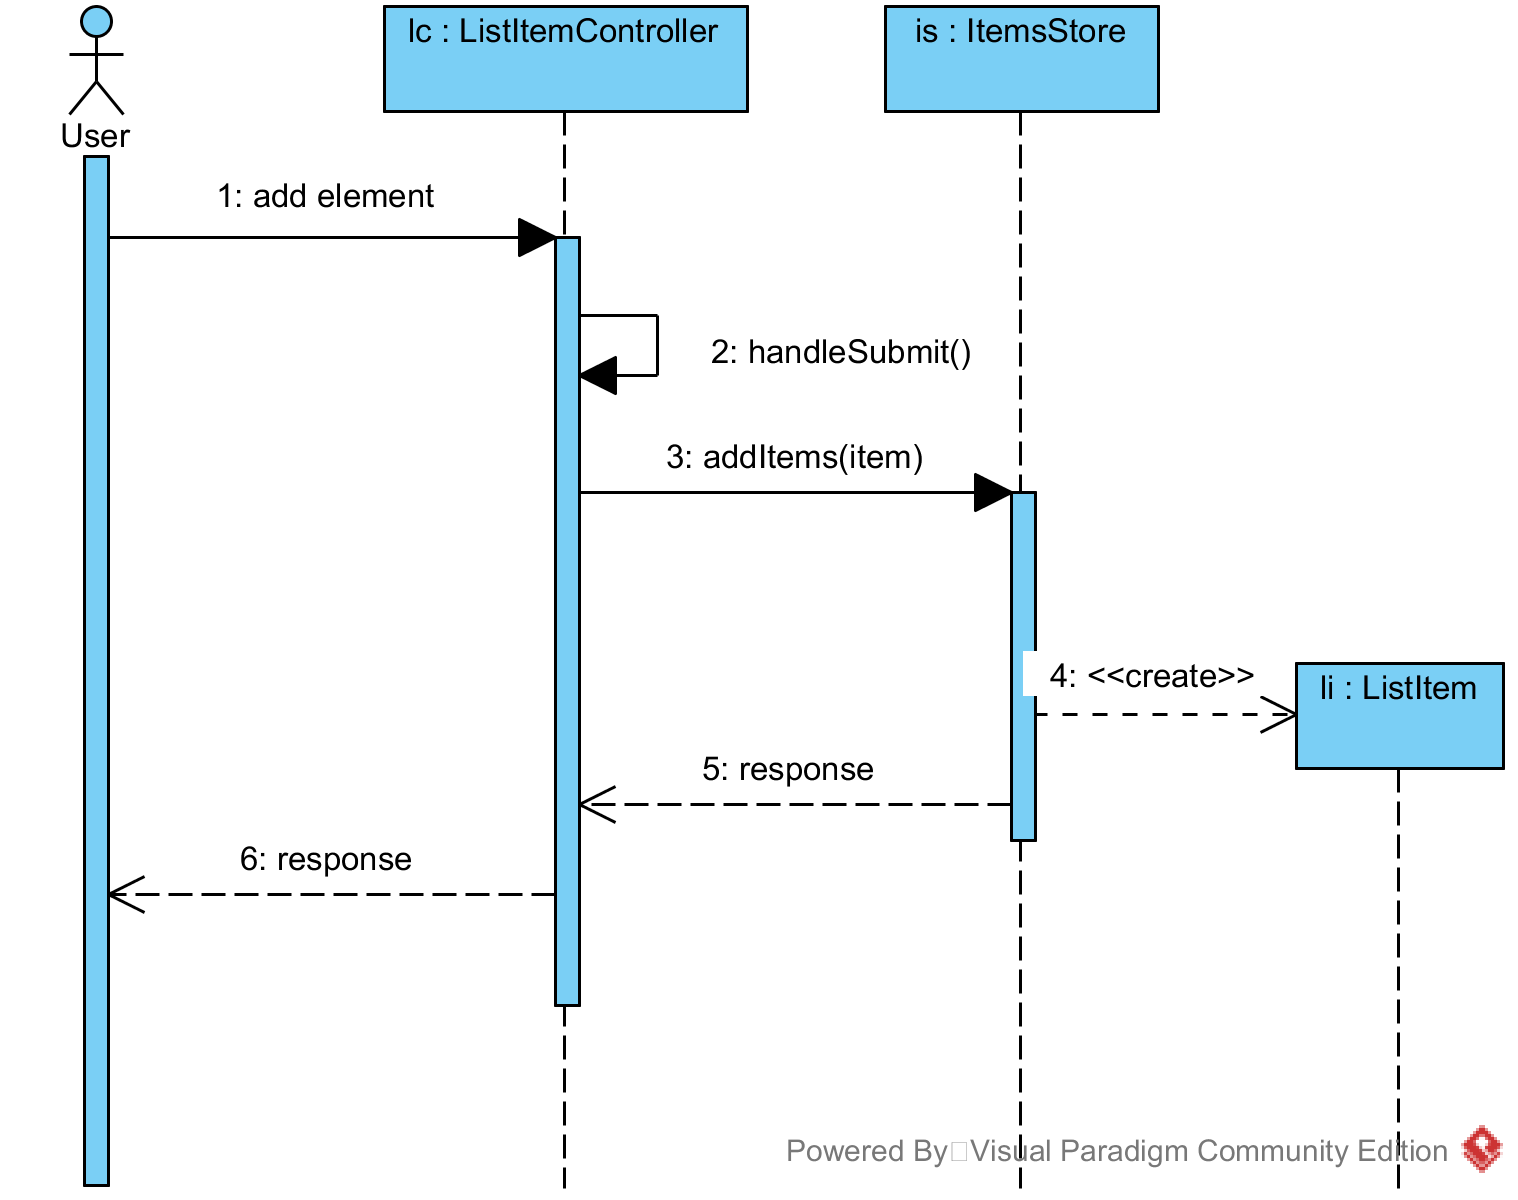
\includegraphics[width=15cm]{./diagrammi/sequenza/aggiunta_elemento_todo.png}
	\caption{Diagramma di sequenza - Aggiunta elemento alla To-do list}
\end{figure}
Lo \textit{User} effettua la richiesta di aggiunta di un elemento, che viene ricevuta dalla classe \code{ListItemController}. La classe quindi invoca il metodo \code{handleSubmit()} che recupera l'oggetto da aggiungere alla lista. Quindi invoca il metodo \code{addItems(item)} della classe \code{ItemsStore}, il quale crea l'oggetto \code{ListItem}.

\subsubsection{Rimozione elemento dalla To-do list}
\begin{figure}[H]
	\centering
	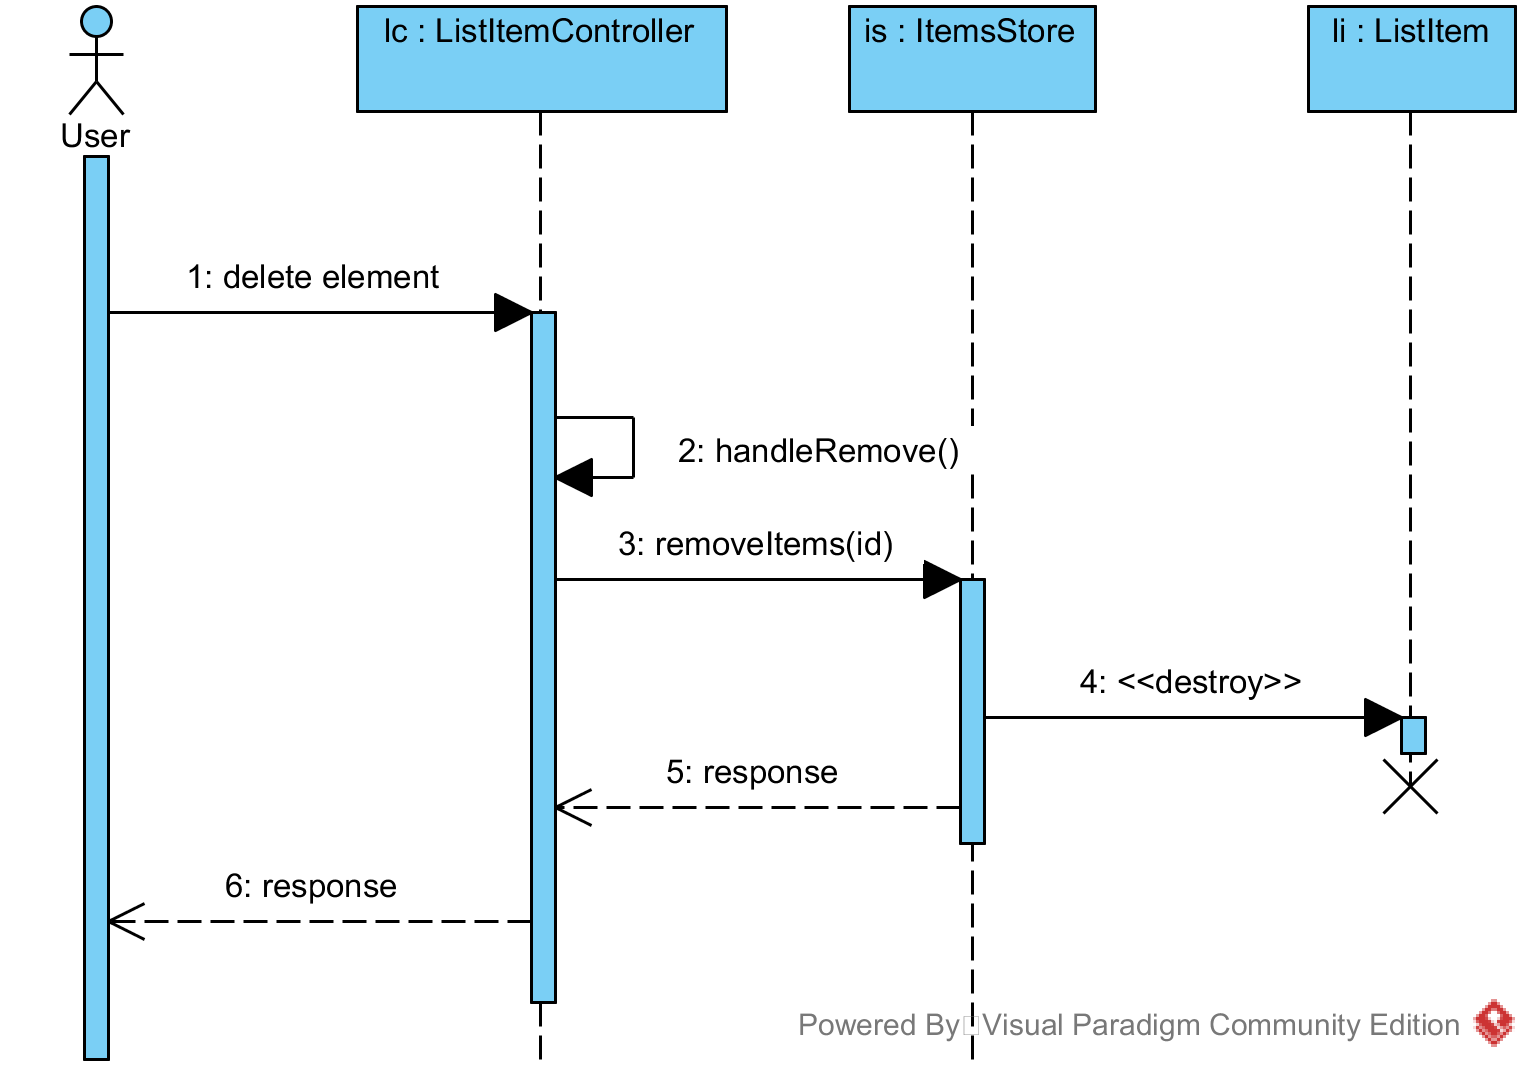
\includegraphics[width=15cm]{./diagrammi/sequenza/rimozione_elemento_todo.png}
	\caption{Diagramma di sequenza - Rimozione elemento dalla To-do list}
\end{figure}
Lo \textit{User} effettua la richiesta di rimozione di un elemento, che viene ricevuta dalla classe \code{ListItemController}. La classe quindi invoca il metodo \code{handleRemove()} che recupera l'id dell'oggetto da rimuovere dalla lista. Quindi invoca il metodo \code{removeItems(id)} della classe \code{ItemsStore}, il quale distrugge l'oggetto \code{ListItem}.

\subsubsection{Completamento elemento dalla To-do list}
\begin{figure}[H]
	\centering
	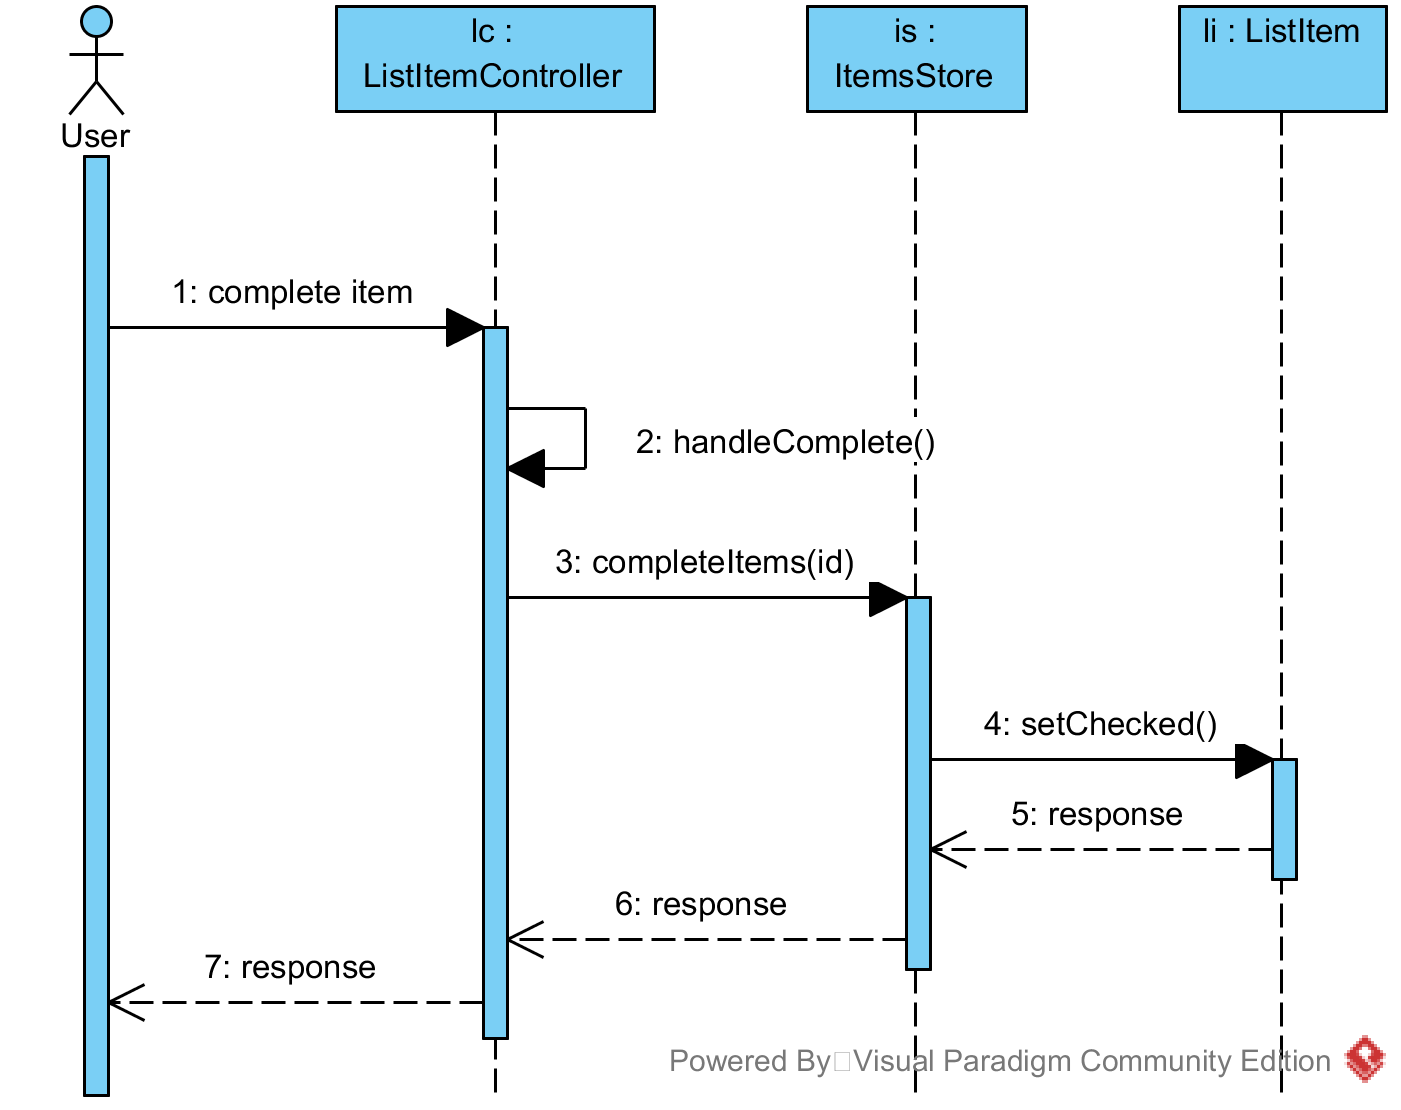
\includegraphics[width=15cm]{./diagrammi/sequenza/completa_elemento_todo.png}
	\caption{Diagramma di sequenza - Completamento elemento dalla To-do list}
\end{figure}
Lo \textit{User} effettua la richiesta di completamento di un elemento, che viene ricevuta dalla classe \code{ListItemController}. La classe quindi invoca il metodo \code{handleComplete()} che recupera l'id dell'oggetto da completare. Quindi invoca il metodo \code{completeItems(id)} della classe \code{ItemsStore}, il quale invoca la funzione \code{setChecked()} che modifica lo stato dell'oggetto \code{ListItem}.

\subsection{\DemoName}
Nello scenario descritto dalla demo, tramite il framework e le bubble da esso prodotte sarà possibile per gli attori interagire con il sistema nei seguenti modi, suddivisi per attore che li compie.

\subsubsection{Customer}

\paragraph{Lettura del menu}\mbox{} \\
\nopagebreak
\begin{figure}[H]
	\centering
	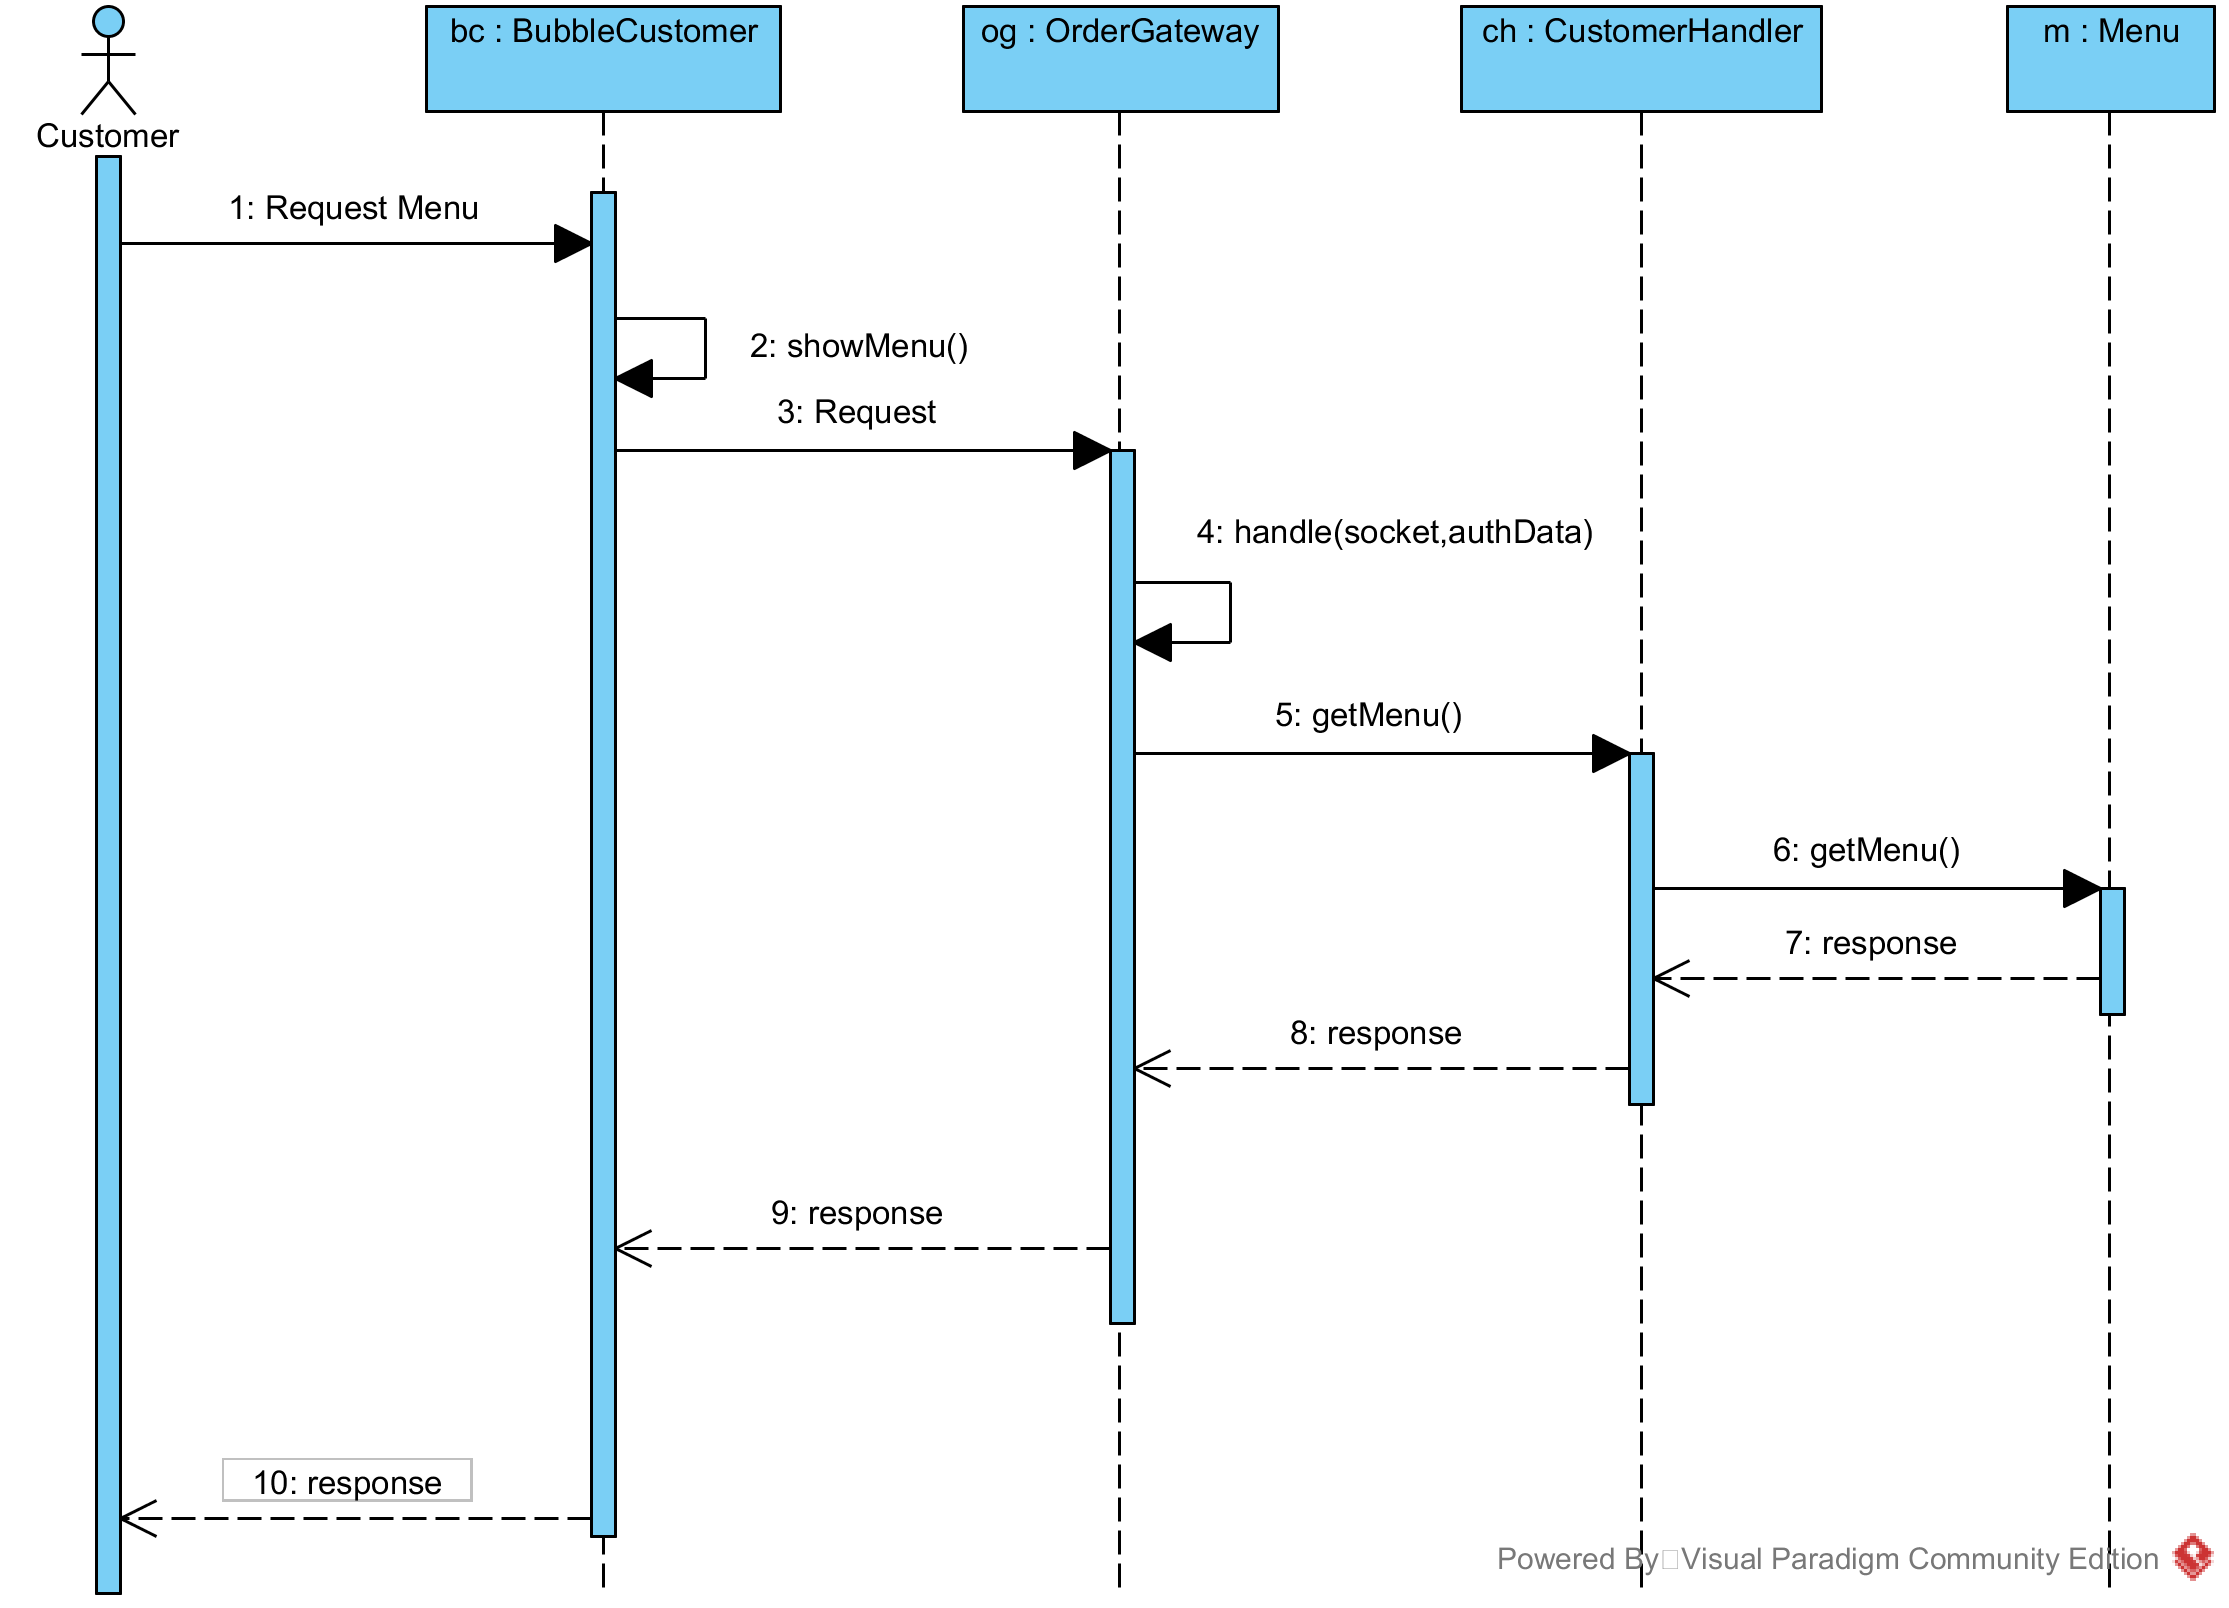
\includegraphics[width=15cm]{./diagrammi/sequenza/letturadelmenu.png}
	\caption{Diagramma di sequenza - Lettura del menu}
\end{figure}
Il \textit{Customer} effettua la richiesta del menu, che viene ricevuta dalla classe \code{BubbleCustomer}. La classe quindi invoca il metodo \code{showMenu()} che invia la richiesta di visualizzazione del menu all'\code{OrderGateway}. L'\code{OrderGateway} indirizza la richiesta verso l'handler corretto tramite il metodo \code{handle(socket,authData)} e quindi invoca la funzione \code{getMenu()} della classe \code{CustomerHandler}. Il metodo recupera il menu dallo store richiamando la funzione \code{getMenu()} della classe \code{Menu} che restituisce il menu al chiamante.  

\clearpage
\newgeometry{margin=1.5cm}
\paragraph{Effettua ordinazione}\mbox{} \\
\pagestyle{empty}
\begin{figure}[H]
	\centering
	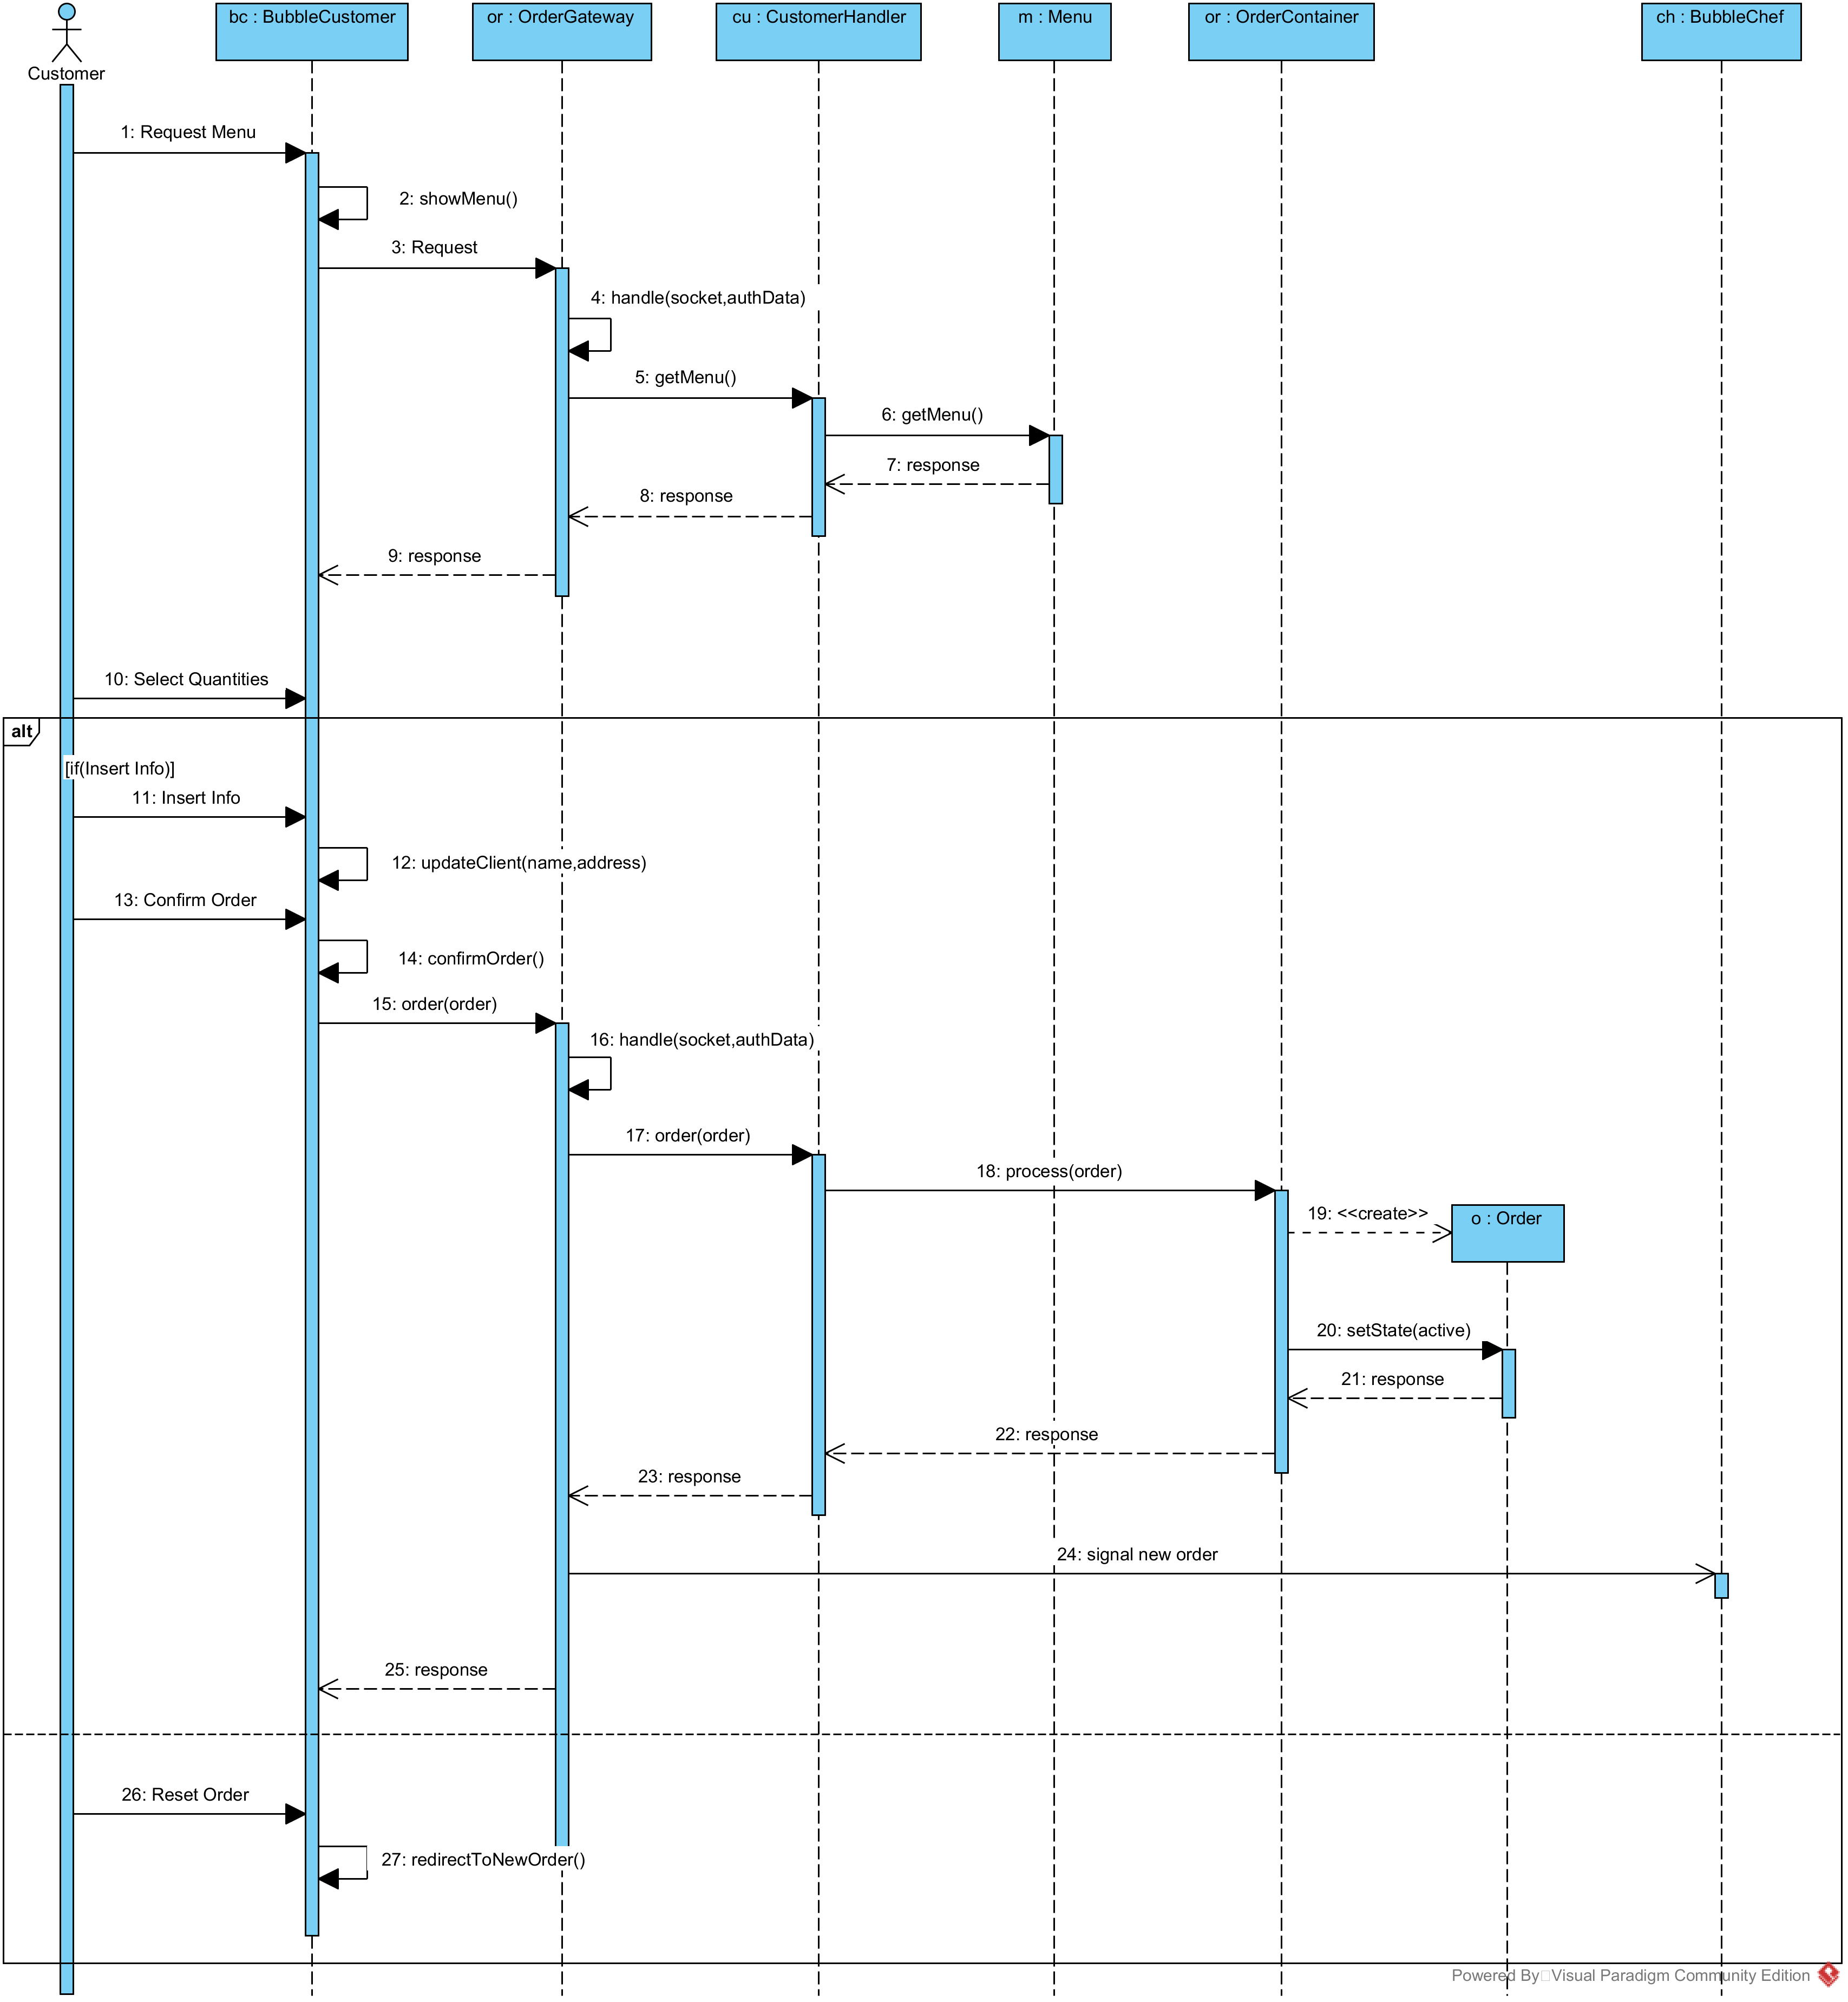
\includegraphics[width=19cm]{./diagrammi/sequenza/faiordinazione.png}
	\caption{Diagramma di sequenza - Effettua ordinazione}
\end{figure}
\restoregeometry
\pagestyle{plain}
Il \textit{Customer} effettua la richiesta del menu seguendo la medesima procedura descritta nel diagramma di sequenza precedente. Una volta ricevuto il menu procede a selezionare le quantità dei diversi prodotti. Una volta selezionati i piatti desiderati e le loro quantità \textit{Customer} ha due scelte: resettare l'ordine, facendo si che la classe \code{BubbleCustomer} lo reindirizzi, tramite il metodo \code{redirectToNewOrder()}, ad una pagina dove può ricominciare a creare l'ordine da zero; inserire il nome e l'indirizzo, che vengono ricevuti e memorizzati dalla classe \code{BubbleCustomer} tramite il metodo \code{updateClient(name, address)}. Se ha scelto la seconda opzione l'utente può procedere alla conferma dell'ordine che viene ricevuta dalla classe \code{BubbleCustomer}. La classe invoca il metodo \code{confirmOrder()} che invia la richiesta dell'ordine all'\code{OrderGateway}, il quale tramite la funzione \code{handle(socket,authData)} la reindirizza a \code{CustomerHandler} invocando la funzione \code{order(order)}. Il metodo processa l’ordine confermato dal Customer e gli assegna un id. A questo punto chiama la funzione \code{process(order)} della classe \code{OrderContainer} che completa la costruzione dell'ordine e lo rende attivo con \code{setState(active)}. L'\code{OrderGateway} si preoccupa a questo punto di avvisare lo \textit{Chef} dell'esistenza di un nuovo ordine mandando un segnale alla classe \code{BubbleChef}  

\subsubsection{Chef}

\paragraph{Segnalazione piatto pronto}\mbox{} \\
\nopagebreak
\begin{figure}[H]
	\centering
	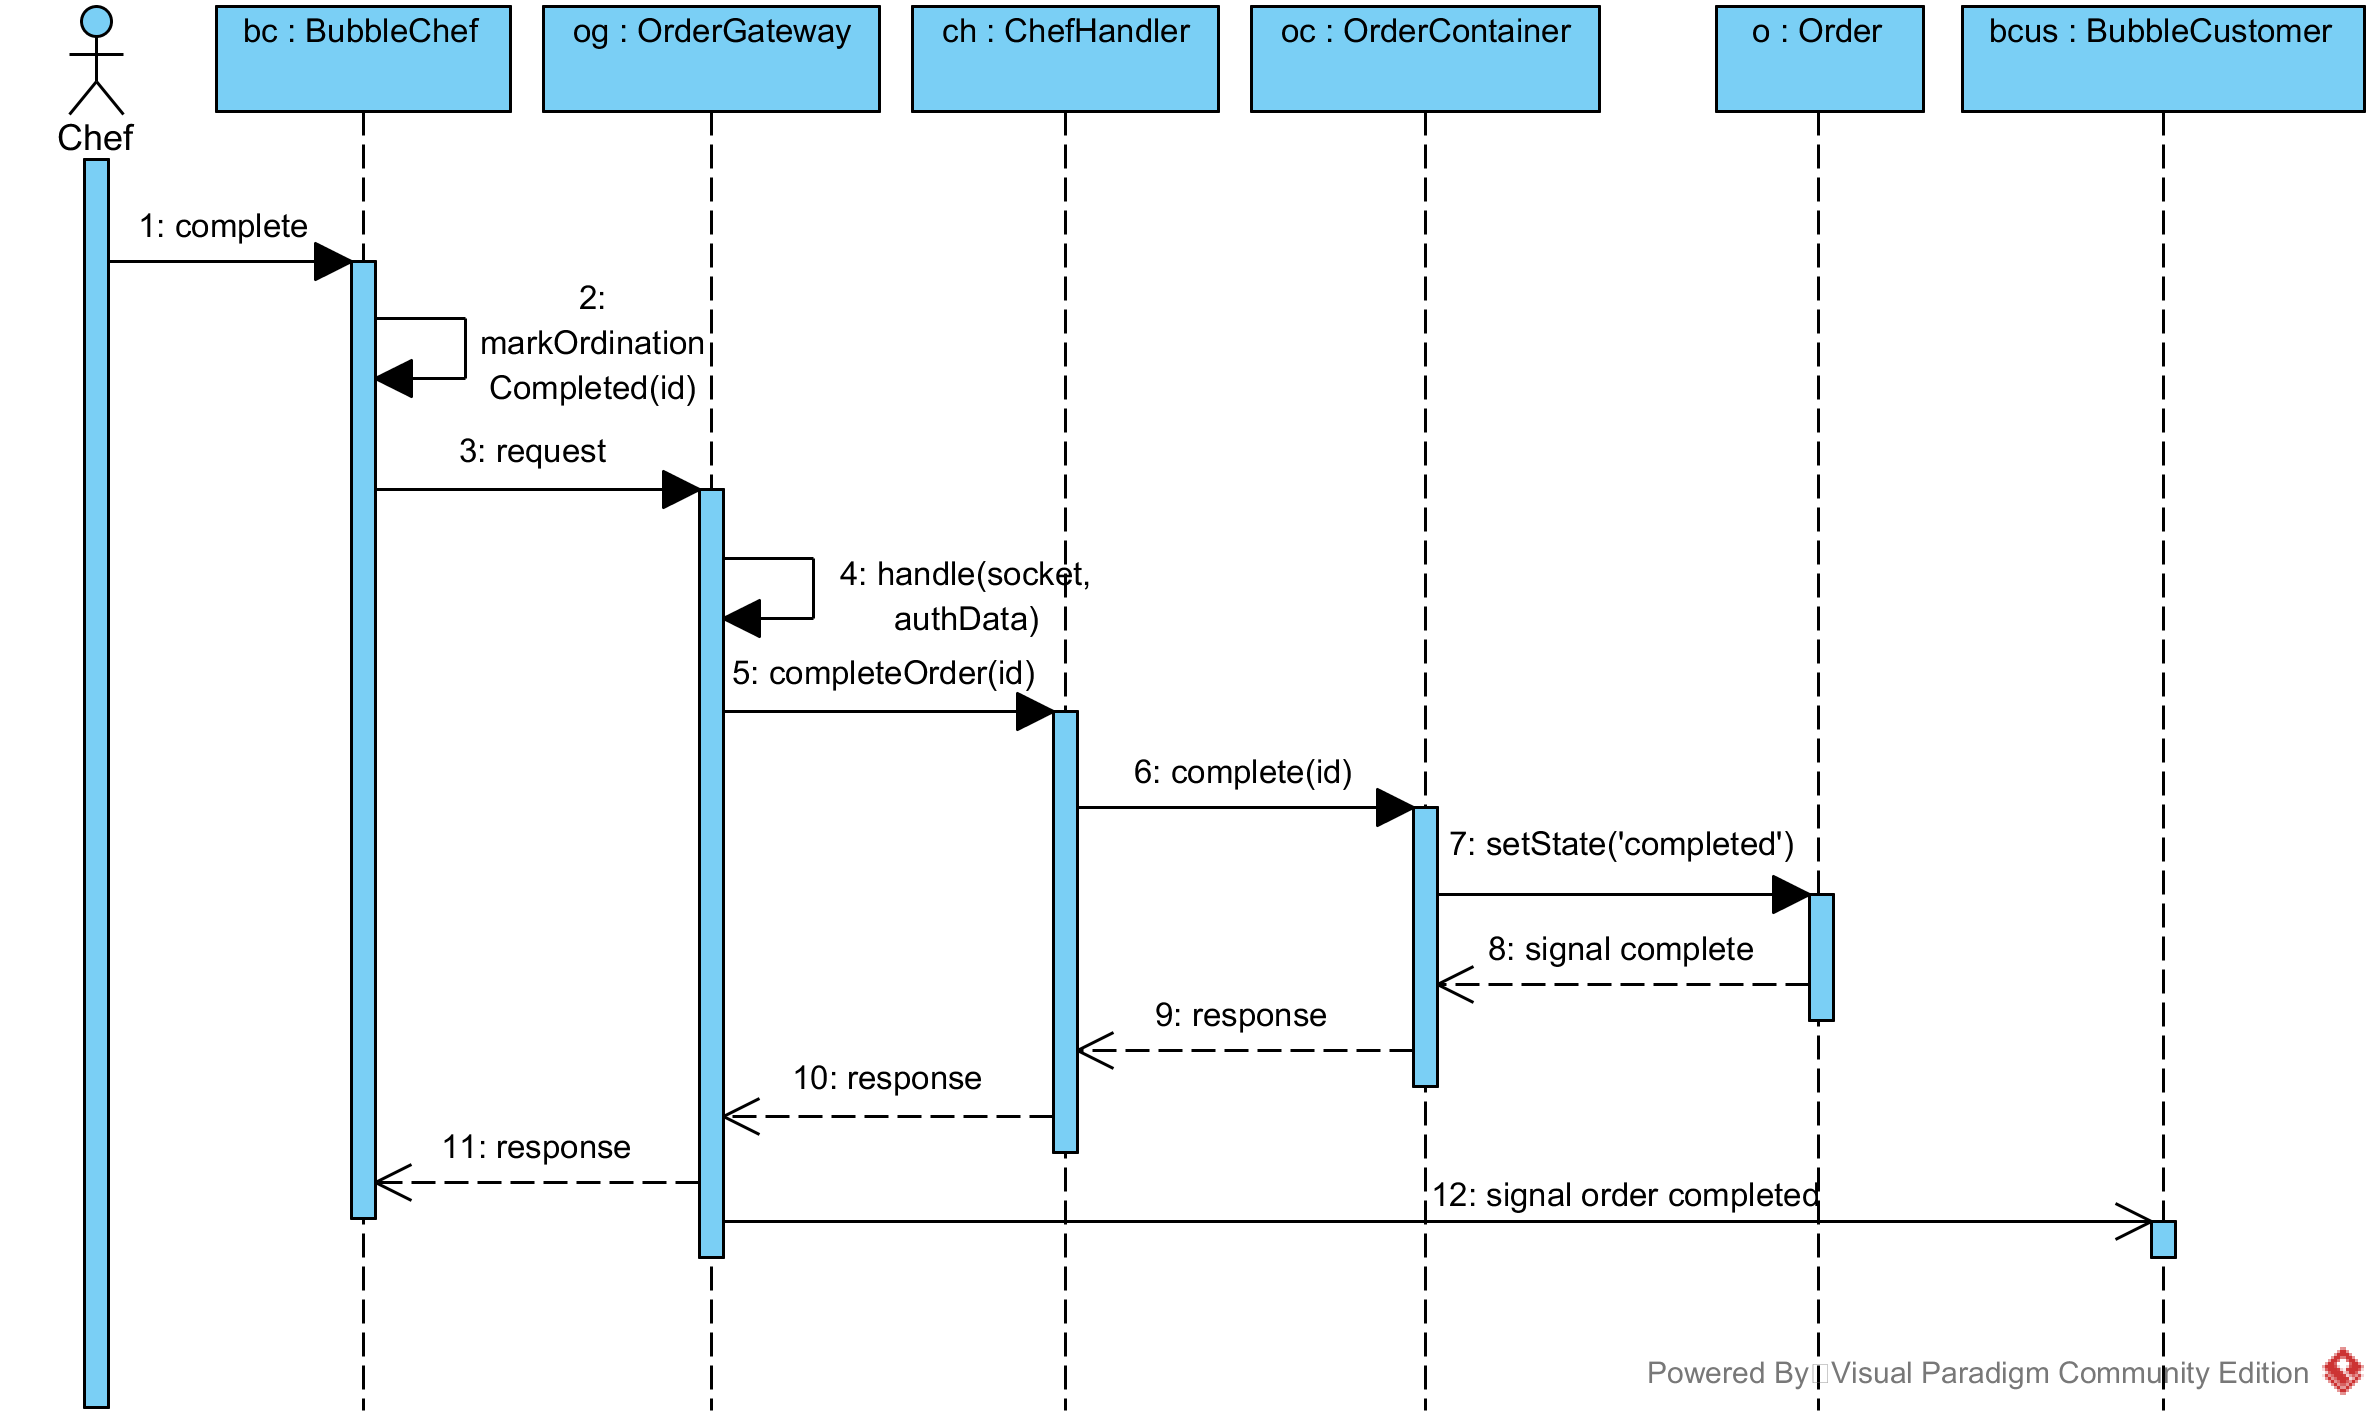
\includegraphics[width=15cm]{./diagrammi/sequenza/chef_piatto_pronto.png}
	\caption{Diagramma di sequenza - Segnalazione piatto pronto}
\end{figure}
Lo \textit{Chef} completa un piatto da preparare e la classe \code{BubbleChef}, la quale indica come completata l'ordinazione tramite il metodo \code{markOrdinationCompleted(id)} e invia una richiesta all'\code{OrderGateway}. L'\code{OrderGateway} reindirizza la richiesta tramite il metodo \code{handle(socket,authData)} e invoca il metodo \code{completeOrder(id)} della classe \code{ChefHandler}. La funzione salva l'ordine completato richiamando il metodo \code{complete(id)} della classe \code{OrderContainer}, che completa l'ordine e ne aggiorna lo stato tramite il metodo \code{setState("completed")} della classe \code{Order}. A questo punto la classe \code{OrderGateway} segnala a \code{BubbleCustomer} il completamento dell'ordine.

\subsubsection{Manager}

\paragraph{Visualizza menu}\mbox{} \\
\nopagebreak
\begin{figure}[H]
	\centering
	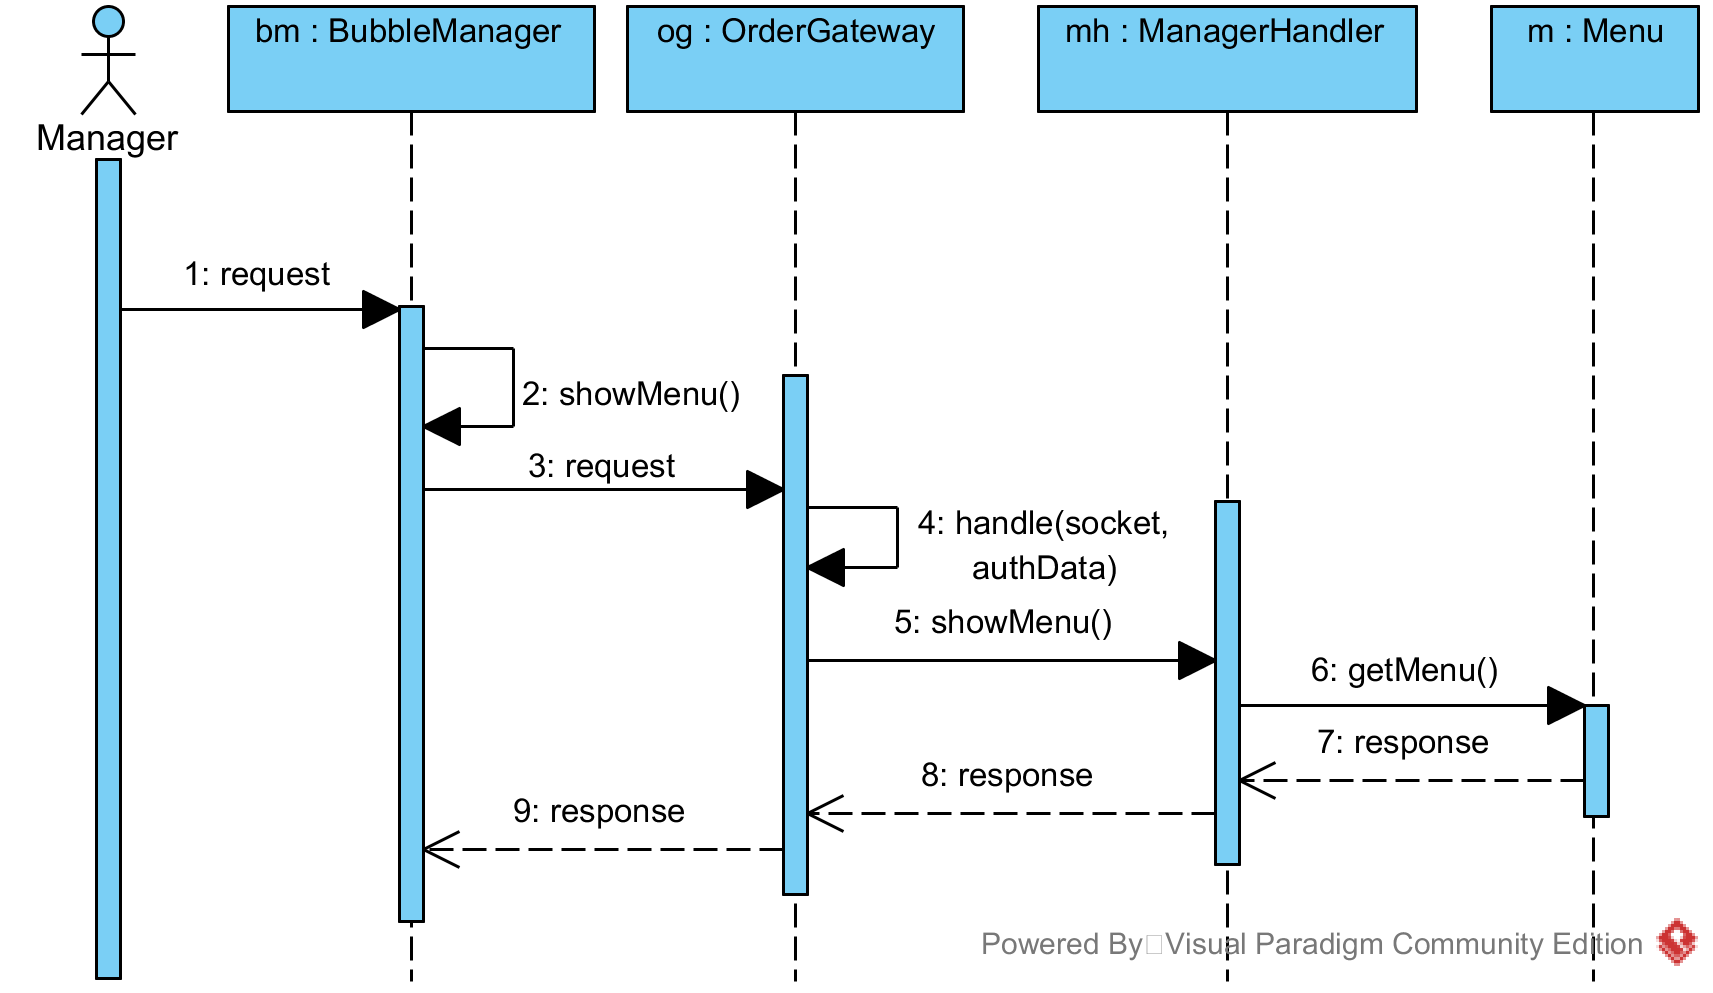
\includegraphics[width=15cm]{./diagrammi/sequenza/visualizza_menu.png}
	\caption{Diagramma di sequenza - Visualizza menu}
\end{figure}
Il \textit{Manager} richiede di visualizzare il menu alla classe \code{BubbleManager}, la quale invoca il metodo \code{showMenu()} che invia la richiesta di un menu aggiornato a \code{OrderGateway}. \code{OrderGateway} inoltra la risposta tramite il metodo \code{handle(socket, authData)} e quindi invoca il metodo \code{showMenu()} della classe \code{ManagerHandler}. Il metodo recupera il menu tramite l'invocazione della funzione \code{getMenu()} della classe \code{Menu} la quale gli restituisce il menu aggiornato.

\paragraph{Modifica menu - aggiunta}\mbox{} \\
\nopagebreak
\begin{figure}[H]
	\centering
	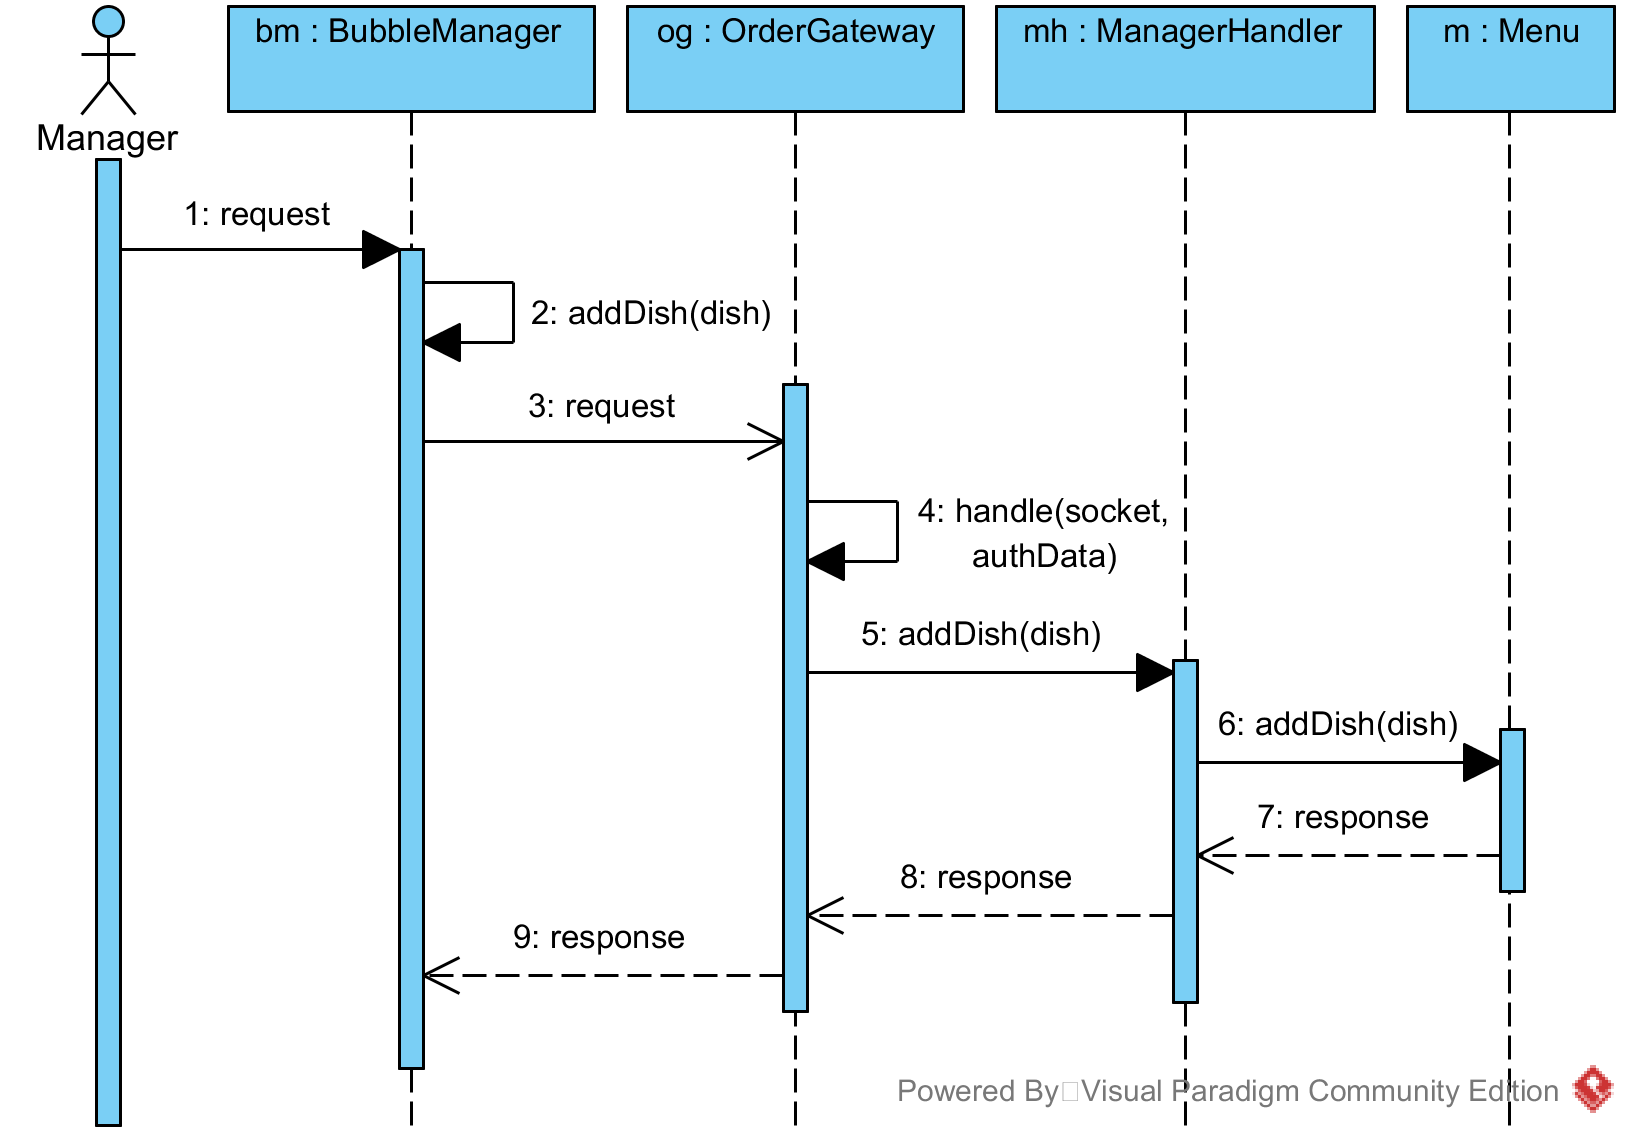
\includegraphics[width=15cm]{./diagrammi/sequenza/modifica_menu_add.png}
	\caption{Diagramma di sequenza - Modifica menu - aggiunta}
\end{figure}
Il \textit{Manager} richiede l'aggiunta di un piatto alla classe \code{BubbleManager}. La classe invoca il metodo \code{addDish(dish)} il quale segnala la richiesta a \code{OrderGateway} che la reindirizza tramite il metodo \code{handle(socket,authData)} e invoca il metodo \code{addDish(dish)} della classe \code{ManagerHandler}. La funzione aggiunge quindi il piatto al menu richiamando il metodo \code{addDish(dish)} della classe \code{Menu}.

\paragraph{Modifica menu - edit}\mbox{} \\
\nopagebreak
\begin{figure}[H]
	\centering
	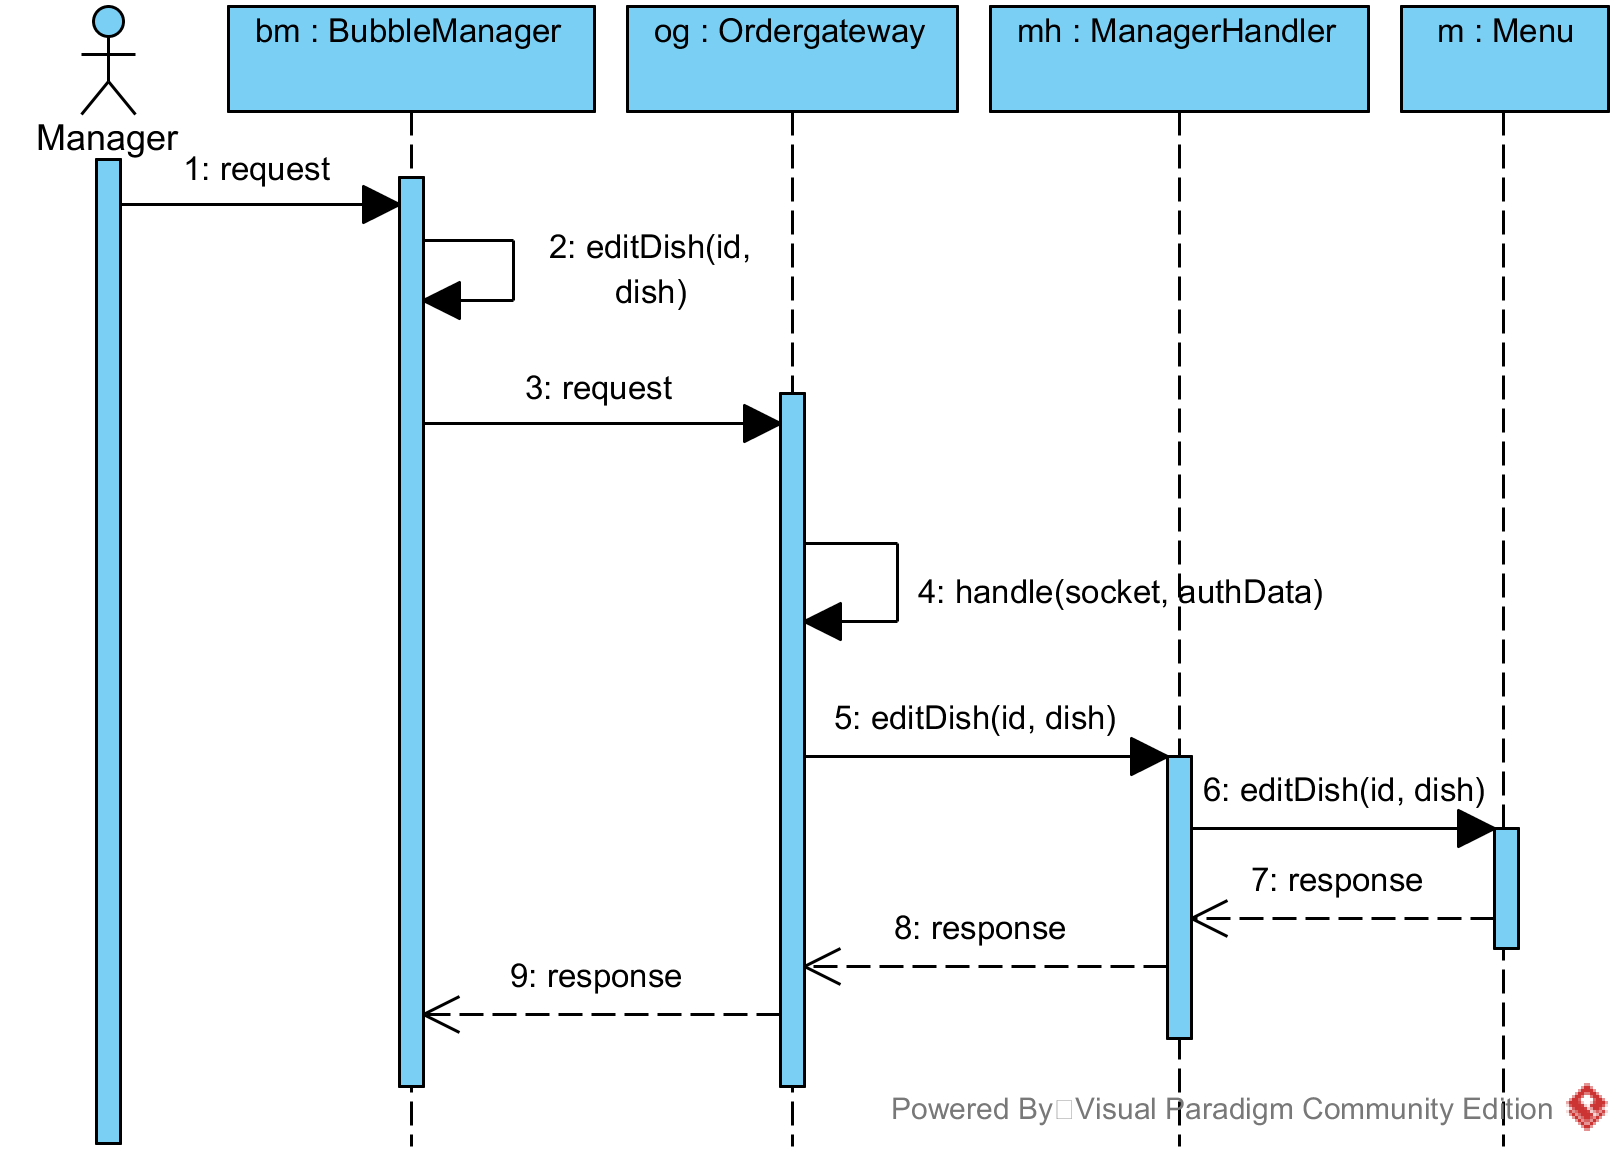
\includegraphics[width=15cm]{./diagrammi/sequenza/modifica_menu_edit.png}
	\caption{Diagramma di sequenza - Modifica menu - edit}
\end{figure}
Il \textit{Manager} richiede la modifica di un piatto del menu alla classe \code{BubbleManager}. La classe invoca il metodo \code{editDish(id,dish)} il quale segnala la richiesta di modifica a \code{OrderGateway} che viene reindirizza tramite il metodo \code{handle(socket,authData)}. \code{OrderGateway} quindi invoca il metodo \code{editDish(id,dish)} della classe \code{ManagerHandler} il quale modifica il piatto del menu richiamando la funzione \code{editDish(id,dish)} della classe \code{Menu}.

\paragraph{Modifica menu - rimozione}\mbox{} \\
\nopagebreak
\begin{figure}[H]
	\centering
	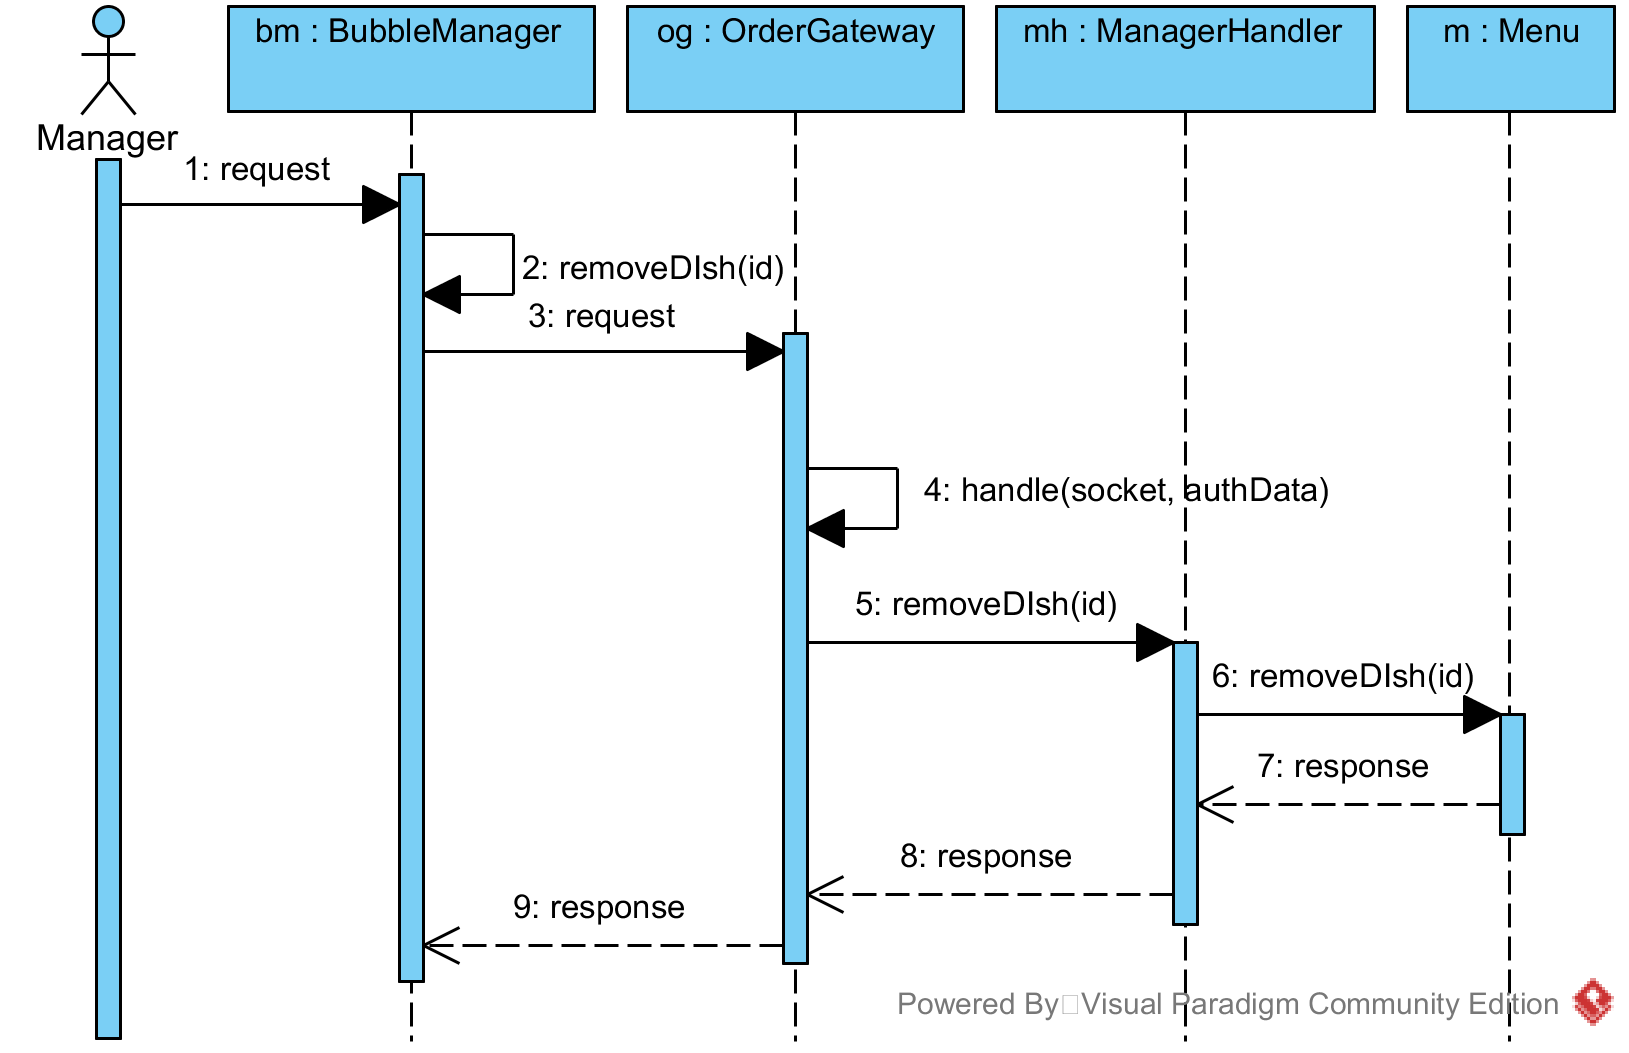
\includegraphics[width=15cm]{./diagrammi/sequenza/modifica_menu_delete.png}
	\caption{Diagramma di sequenza - Modifica menu - rimozione}
\end{figure}
Il \textit{Manager} richiede la rimozione di un piatto del menu alla classe \code{BubbleManager}. La classe invoca il metodo \code{removeDish(id)} il quale segnala la richiesta di rimozione a \code{OrderGateway} che la reindirizza tramite il metodo \code{handle(socket,authData)} e invoca il metodo \code{removeDish(id)} della classe \code{ManagerHandler}. La funzione aggiunge quindi il piatto al menu richiamando il metodo \code{removeDish(id)} della classe \code{Menu}.

\paragraph{Visualizza ordini}\mbox{} \\
\nopagebreak
\begin{figure}[H]
	\centering
	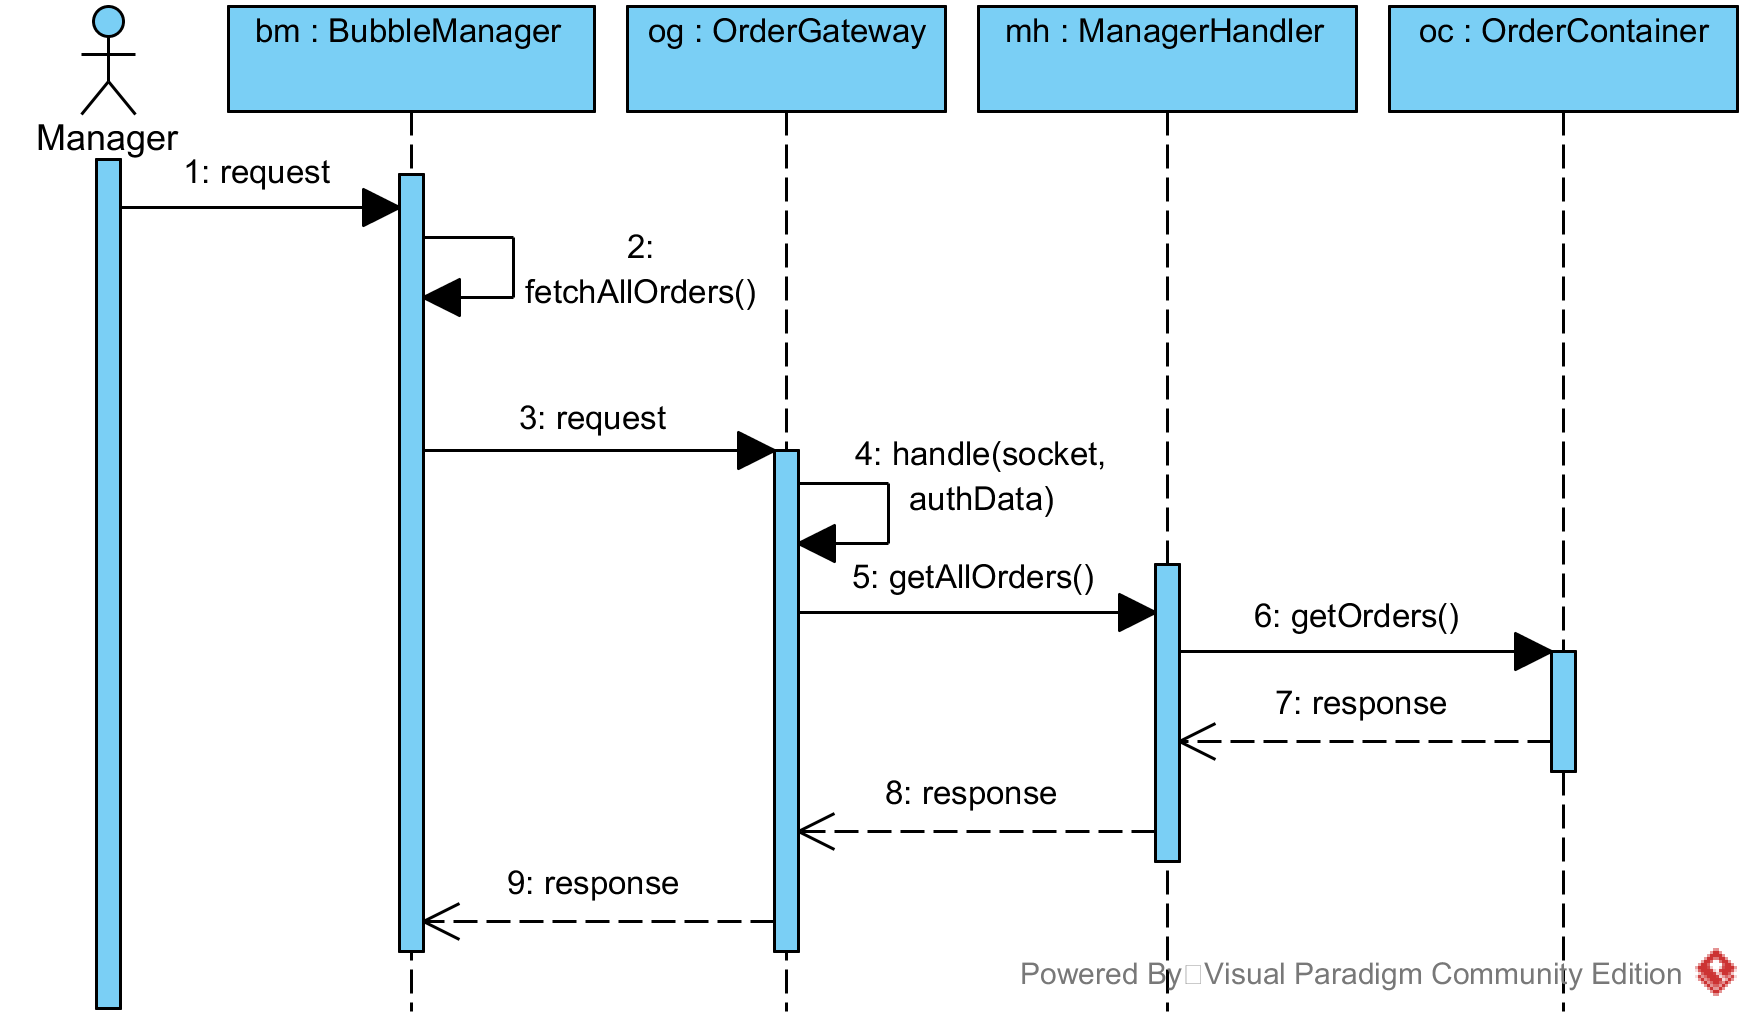
\includegraphics[width=15cm]{./diagrammi/sequenza/visualizza_ordini.png}
	\caption{Diagramma di sequenza - Visualizza ordini}
\end{figure}
Il \textit{Manager} effettua la richiesta di visualizzazione degli ordini, che viene ricevuta dalla classe \code{BubbleManager}. \code{BubbleManager} quindi invoca il metodo \code{fetchAllOrders()} che invia una richiesta alla classe \code{OrderGateway} per ricevere il contenitore degli ordini aggiornato. \code{OrderGateway} reindirizza la richiesta tramite il metodo \code{handle(socket,authData)} e invoca la funzione \code{getAllOrders()} della classe \code{ManagerHandler} la quale recupera tutti gli ordini presenti tramite il metodo \code{getOrders()} della classe \code{OrderContainer}.

\paragraph{Elimina ordine}\mbox{} \\
\nopagebreak
\begin{figure}[H]
	\centering
	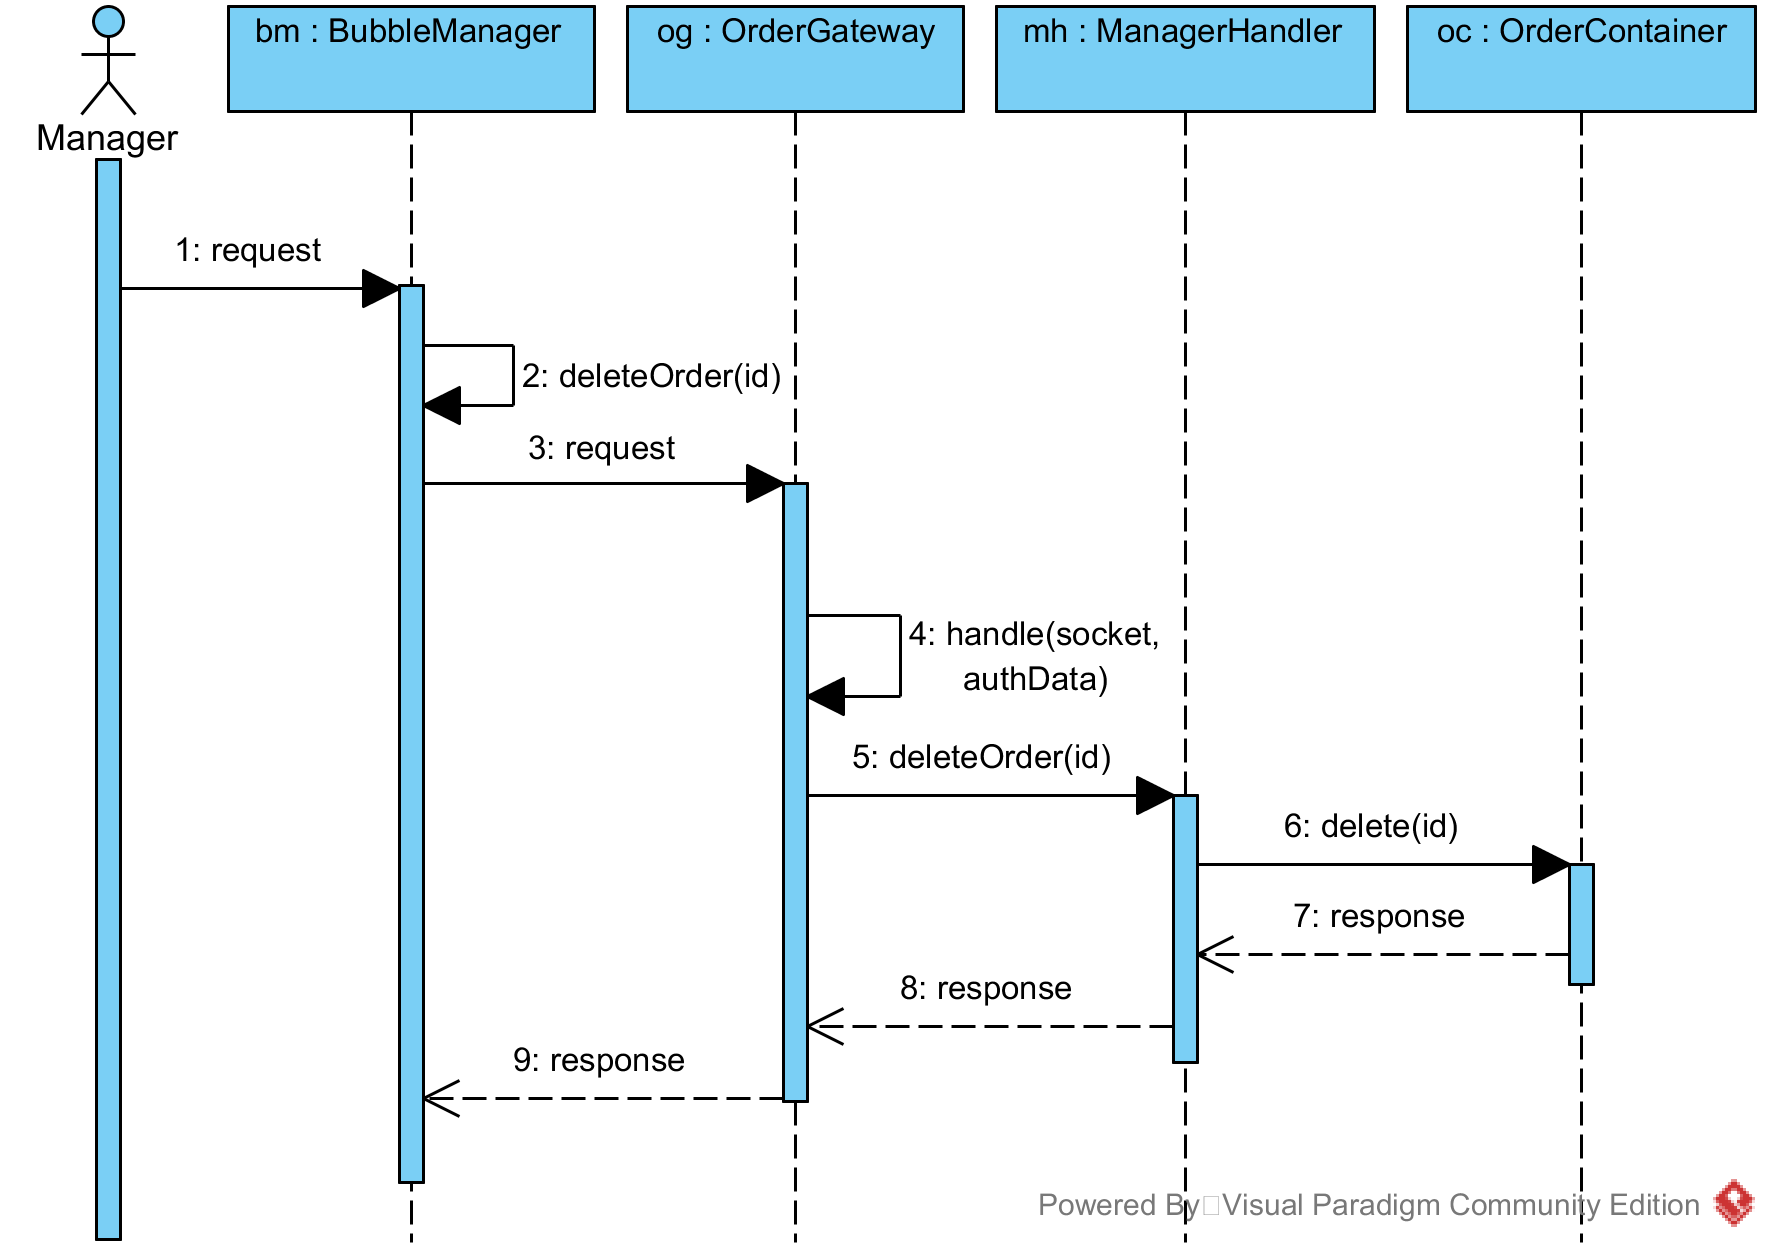
\includegraphics[width=15cm]{./diagrammi/sequenza/elimina_ordine.png}
	\caption{Diagramma di sequenza - Elimina ordine}
\end{figure}
Il \textit{Manager} richiede l'eliminazione di un ordine alla classe \code{BubbleManager}, la quale invoca il metodo \code{deleteOrder(id)} che segnala la richiesta all'\code{OrderContainer}. \code{OrderContainer} reindirizza la richiesta tramite il metodo \code{handle(socket,authData)} e invoca il metodo \code{deleteOrder(id)} della classe \code{ManagerHandler} il quale elimina l'ordine invocando la funzione \code{delete(id)} della classe \code{OrderContainer}.